% !TEX root = ../../handbook-physics.tex
%!TEX TS-program = pdflatex
%!TEX encoding = UTF-8 Unicode


%\documentclass{article}
%\usepackage[svgnames]{xcolor}
%\usepackage{tikz}
%\usepackage{amsmath}
%\usepackage{physics}
%
%\begin{document}
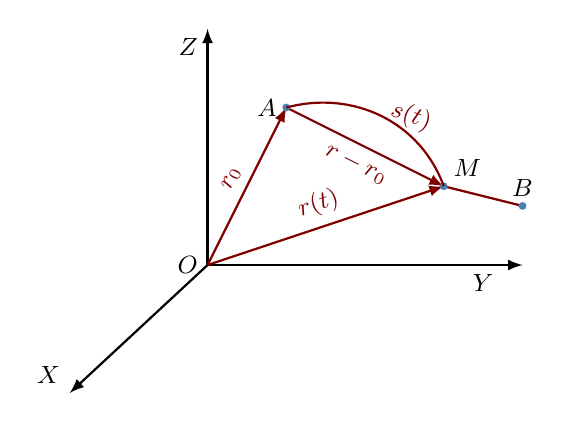
\begin{tikzpicture}[scale=0.5,font=\small]
%\draw [help lines] (0,0) grid (5,5);
		
		\draw [thick,latex-](0,6) to (0,0);
		\draw [thick,-latex](0,0) to (-3.5, -3.25);
		\draw [thick,-latex](0,0) to (8,0);
		\draw [thick,-latex,Maroon](0,0) -- (2, 4)node [midway, above, sloped] (TextNode){$\vb{r_{0}}$} ;
		
		\draw [thick,-latex,Maroon](0,0) -- (6, 2)node [midway, above, sloped] (TextNode){$\vb{r}(t)$} ;
		\draw [thick,-latex,Maroon](2,4) -- (6, 2)node [midway, below, sloped] (TextNode){$\vb{r-r_{0}}$} ;
			\draw [thick,Maroon] (8,1.5)-- (6, 2);
	 	\node [left] at (2,4) {$A$};

	 	\node [above] at (8,1.5) {$B$};
	\fill [SteelBlue] (2,4) circle [radius=0.1];;	
	\fill [SteelBlue] (6,2) circle [radius=0.1];;
	\fill [SteelBlue] (8,1.5) circle [radius=0.1];;
		\node [above right] at (6,2) {$M$};
		\node [left] at (0,0) {$O$};
		\node [below left] at (0,6) {$Z$};
		\node [above left] at (-3.5, -3.25) {$X$};
		\node [below] at (7, 0) {$Y$};
\draw[thick,Maroon] (2,4) to [out=15,in=110] (6,2);
\node [above right,rotate=-20,Maroon] at (4.25,3.5){$s(t)$};
	%	\node [left] at (1,2) {$\vb{r_{0}}$};
%		\node [above] at (3,1) {$\vb{r(t)}$};
%		\node [above] at (4, 3) {$M (x,y,z)$};
	\end{tikzpicture}
%\end{document}